% !TEX root = ../Dokumentation.tex

\section{Bedienung der Applikation}\label{sec:BedienungApplikation}
Der gesamte Projektquellcode ist auf GitHub öffentlich verfügbar\footnote{Das Projekt ist unter https://github.com/aoezd/Virtual-Reality-Praktikum aufrufbar.} und kann als ZIP-Datei in ein beliebiges Ordner heruntergeladen werden. Es wird empfohlen unter einem Linux-System zu testen, da im Projekt ein Makefile mitgeliefert wird. Das \acs{lst} \ref{lst:projectstructure} beschreibt die Projektstruktur.

\begin{lstlisting}[caption={Die Beschreibung der allgemeinen Projektstruktur}, label={lst:projectstructure}]
- Application/
  -- Header/
    --- // Wie Source-Ordner nur mit Header-Dateien
  -- Images/
    --- CameraCalibration/
      ---- // Bilder mit Kalibriermuster, die im Rahmen der Live-Kalibrierung gemacht wurden
    --- chessboard.png // Kalibriermuster
    --- markerCoin.jpg // Standard-Marker für die Münze
    --- markerObstacle.jpg // Standard-Marker für die Hindernisse
    --- markerPlayer.jpg // Standard-Marker für den Spieler
  -- Resources/
    --- Logitech720p.ccc // Kalibrierungdatei die im Rahmen der Entwicklung verwendet wurde
  -- Source/
    --- ImageDetection/
      ---- camera.cpp
      ---- detectormarkerbased.cpp
    --- Logging/
      ---- logger.cpp
    --- Rendering3D/
      ---- rendering3d.cpp
    --- Utilities/
      ---- algebra.cpp
      ---- argparse.cpp
      ---- imageio.cpp
      ---- utils.cpp
    --- main.cpp
  -- Makefile
- Test/
  -- Header/
    --- catch.h // Header-only test framework für C++ Applikationen; https://github.com/philsquared/Catch
  -- Source/
    -- // Wie ../Application/Source-Ordner nur mit C++-Dateien die getestet wurden
\end{lstlisting}

\noindent Um die Applikation starten zu können, muss ein Terminal im Projektunterordner \glqq Application/\grqq{} geöffnet und mit dem Kommando \glqq \texttt{make}\grqq{} die Applikation gebaut werden. Je nachdem welche Version von OpenCV/OpenGL installiert ist bzw. wo diese Bibliotheken im jeweiligen System installiert sind, kann es sein, dass Pfade zu Header-Dateien im Quellcode angepasst werden müssen. Nachdem die Applikation erfolgreich gebaut wurde, kann diese mit den folgenden Eingabeparametern gestartet werden:

\begin{itemize}
    \item \texttt{-h, --help}: Spielt die Bedienungsanleitung auf der Konsole aus
    \item \texttt{-mc, --markercoin [Pfad zum Markerbild]}: Definiert den Marker für das Objekt einer Münze. Standardmäßiger Marker: \glqq \texttt{Application/Images/markerCoin.jpg}\grqq
    \item \texttt{-mo, --markerobstacle [Pfad zum Markerbild]}: Definiert den Marker für das Objekt eines Hindernisses. Standardmäßiger Marker: \glqq \texttt{Application/Images/markerObstacle.jpg}\grqq
    \item \texttt{-mp, --markerplayer [Pfad zum Markerbild]}: Definiert den Marker für das Objekt des Spielers. Standardmäßiger Marker: \glqq \texttt{Application/Images/markerPlayer.jpg}\grqq
    \item \texttt{-ccc, --cameracalibrationcompute [Pfad zum Ordner mit Kalibrierungsbildern]}: Berechnet die Kamerakalibrierung anhand der Bilder die im übergebenen Ordner
    \item \texttt{-ccl, --cameracalibrationload [Pfad zur Kalibrierungsdatei]}: Lädt die Kamerakalibrierung aus der übergebenen Datei.
\end{itemize}

\noindent Falls die Applikation ohne die Angabe eines Eingabeparameters ausgeführt wird, startet eine Live-Kamerakalibrierung (\acs{s} \acs{abs} \ref{sssec:kaliRuntime}) automatisch und als Standard definierte Marker werden geladen. Mithilfe der Taste \glqq \texttt{h}\grqq{} können zur Laufzeit weitere Informationen ausgespielt werden (\acs{s} \acs{abb} \ref{fig:HelpShow}).

\begin{figure}[H]
\centering
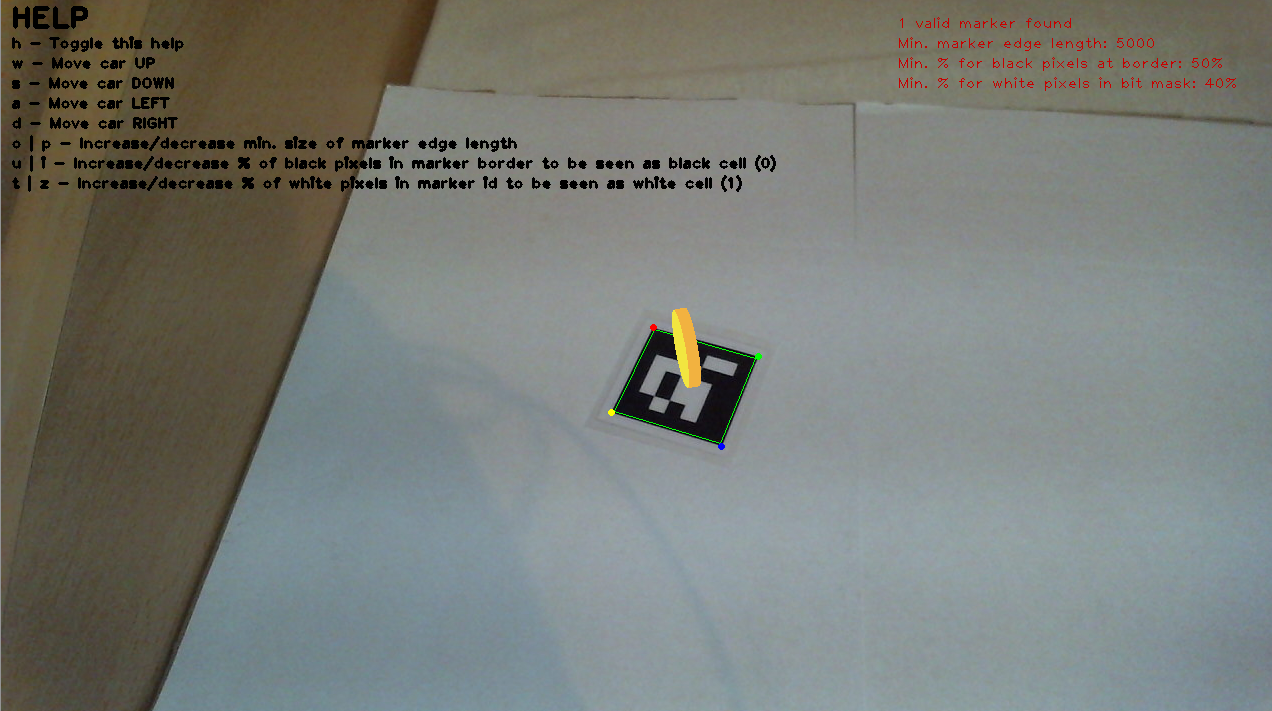
\includegraphics[width=13cm]{Bilder/BedienungDerApplikation/Hilfe.png}
\caption{Darstellung der Hilfeausgabe zur Laufzeit}
\label{fig:HelpShow}
\end{figure}

\subsection{Systemeinstellungen zurzeit der Entwicklung}
Die Applikation wurde auf einem System mit folgenden Eigenschaften entwickelt und getestet:

\begin{table}[H]
\centering
\begin{tabular}{|p{6cm}|p{9cm}|}
\hline
\textbf{Komponente} & \textbf{Beschreibung} \\
\hline
\verb|System| & Linux\\
\hline
\verb|Betriebssystem| & Xubuntu 16.04\\
\hline
\verb|Grafikkarte| & NVIDIA GeForce GTX 970\\
\hline
\verb|Physischer Speicher| & 16 GB \\
\hline
\verb|Grafikkartenspeicher| & 3.5 GB\\
\hline
\verb|OpenGL-Version| & 3.3\\
\hline
\verb|OpenCV-Version| & 3.1.0\\
\hline
\end{tabular}
\caption{Beschreibung der Systemeinstellungen zurzeit der Entwicklung}
\label{tab:SystemSettings}
\end{table}

\newpage
